\section{系统设计}

\subsection{架构概览}

图~\ref{fig:architecture}展示了EdgeSched的整体架构。系统采用分层设计，自上而下分为表示层、领域层、控制面、执行层和数据适配层。用户请求通过WebSocket接口进入系统，经领域层业务逻辑处理后，由控制面统一路由到相应的执行组件。

\begin{figure}[htbp]
\centering
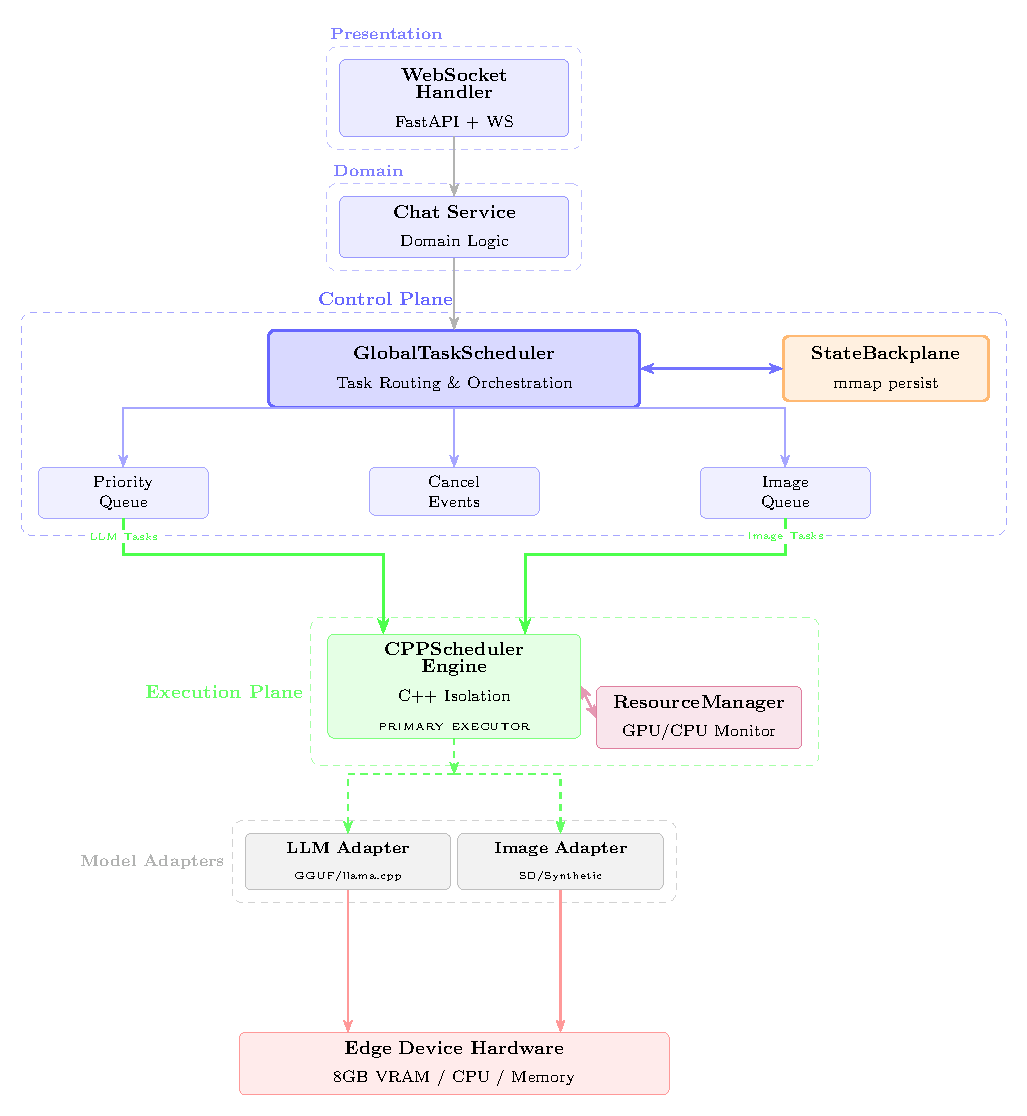
\includegraphics[width=\columnwidth]{../thesis_materials/figures/system_architecture.pdf}
\caption{EdgeSched系统架构}
\label{fig:architecture}
\end{figure}

控制面包含三个核心组件：
\begin{enumerate}
\item \textbf{GlobalTaskScheduler}作为L1路由层，负责任务分发，管理优先级队列、取消事件和图像任务背压控制
\item \textbf{CPPSchedulerEngine}作为L2高性能执行层，封装llama-cpp-python推理引擎，实现GPU/CPU动态资源迁移
\item \textbf{StateBackplane}基于mmap实现零拷贝状态持久化，支持崩溃后12ms内恢复任务状态
\end{enumerate}

执行层包含ResourceManager，负责协调模型生命周期和GPU/CPU资源分配，仲裁多模型间的资源竞争。数据适配层包含LLM Adapter和Image Adapter，分别封装大语言模型（GGUF格式）和图像生成模型（Stable Diffusion）的推理逻辑，屏蔽底层推理引擎的差异，支持多种后端无缝切换。

\subsection{双任务调度}

EdgeSched针对边缘设备上最常见的两类大模型应用——对话交互（LLM）与图像生成（Diffusion）——设计双任务调度机制。LLM属于常驻交互任务（Resident），需要持续响应用户输入，优先常驻GPU以保障低延迟；图像生成属于一次性任务（One-shot），计算密集且在CPU上延迟不可接受，工程上必须依赖GPU。

系统采用不同的调度策略处理两类任务。算法~\ref{alg:scheduling}展示了核心调度逻辑。LLM任务通过\texttt{submit\_llm\_task()}直接提交至CPPSchedulerEngine，默认占用GPU资源；图像生成任务通过\texttt{try\_enqueue\_image\_generation()}进入独立的有界队列。当图像任务到达时，若LLM占用GPU显存，系统立即触发动态资源迁移：保存KV Cache后释放显存，供图像任务加载执行。若多个图像任务连续到达，后续任务在队列中排队，队列满时触发背压机制拒绝新任务，避免资源耗尽导致系统崩溃。

\begin{algorithm}[t]
\caption{带背压控制的任务调度}
\label{alg:scheduling}
\begin{algorithmic}[1]
\STATE \textbf{function} \textsc{提交任务}(task)
\IF{task.type == LLM}
    \STATE 提交到CPPSchedulerEngine
    \STATE 默认分配GPU
\ELSIF{task.type == IMAGE}
    \IF{queue.size() $<$ total\_slots}
        \STATE 任务入队
        \IF{LLM在GPU上}
            \STATE 触发\textsc{卸载到CPU}()
        \ENDIF
    \ELSE
        \STATE \textbf{throw} 队列已满错误
    \ENDIF
\ENDIF
\STATE \textbf{end function}
\end{algorithmic}
\end{algorithm}

这种设计确保常驻任务（LLM）的持续可用性，同时为突发任务（图像生成）提供可预测的资源分配策略。


\subsection{动态资源迁移}

边缘设备配备独立显卡时，显存与系统内存通过PCIe总线分离。LLM常驻GPU（含KV Cache约6-7GB）可保障低延迟交互，但8GB显存无法同时容纳LLM与图像生成模型（约6-7GB）。当图像生成任务到达时，必须立即释放LLM占用的显存，否则触发CUDA OOM。此时显存成为硬约束，用户体验退化为软约束——短暂的服务降级优于系统崩溃。反之，当图像任务完成、显存空闲时，将LLM迁回GPU恢复高性能，无需牺牲上下文连续性。这种约束条件的非对称性，决定了下行路径（GPU→CPU）采用紧急模式优先释放资源，上行路径（CPU→GPU）采用原子热切换保障服务可用。

\subsubsection{非对称迁移策略}

\textbf{下行路径（GPU → CPU）：紧急模式}。当图像任务到达时，系统触发紧急迁移以立即释放显存。该模式首先通过\texttt{save\_state()}将KV Cache从显存经PCIe复制到内存（约200-300ms），保留对话上下文；随后立即释放GPU显存，消除显存碎片以避免OOM风险。释放完成后，系统并行启动两个操作：后台加载CPU版LLM（从DDR到DDR，利用Page Cache加速，>20GB/s），以及加载图像生成模型到GPU（从DDR经PCIe到GDDR）。此模式通过短暂的上下文保存延迟，换取显存安全与用户体验的兼顾。

\textbf{上行路径（CPU → GPU）：原子热切换}。当图像任务完成、显存空闲时，系统执行原子热切换以恢复LLM的高性能推理。该模式采用Double Buffering策略：
\begin{enumerate}
\item \textbf{预加载}：首先在GPU上全新加载LLM实例（从DDR经PCIe到GDDR），此时CPU实例仍在服务用户请求（不中断）
\item \textbf{热迁移}：待GPU实例就绪后，立即暂停CPU实例，通过\texttt{save\_state()}提取KV Cache并注入GPU实例（纯内存操作）
\item \textbf{切换与卸载}：最后原子替换实例指针，将新请求路由到GPU实例，并异步卸载CPU实例
\end{enumerate}

此模式将服务中断时间从秒级压缩到毫秒级（仅状态注入耗时），最大化服务可用性。

\subsubsection{实现机制}

非对称迁移的实现依赖三个核心机制：
\begin{enumerate}
\item \textbf{并发控制}：\texttt{asyncio.Lock()}保证实例替换的原子性，避免竞态条件
\item \textbf{状态序列化}：llama-cpp-python提供的\texttt{save\_state()} / \texttt{load\_state()}接口实现KV Cache的跨设备迁移，状态数据经PCIe在显存与内存间传输
\item \textbf{异步清理}：通过\texttt{asyncio.create\_task()}后台释放旧实例，避免阻塞服务
\end{enumerate}

\subsection{背压控制}

图像生成任务计算密集且显存占用大，系统采用有界队列防止资源耗尽。图像队列容量由\texttt{queue\_capacity}（默认8）和\texttt{max\_concurrent}（默认1）共同决定，总槽位数为两者之和（默认9）。其中\texttt{max\_concurrent}表示并发执行数，\texttt{queue\_capacity}表示排队等待数。

队列管理通过\texttt{try\_enqueue\_image\_generation()}实现：系统使用\texttt{asyncio.Queue(maxsize=total\_slots)}创建有界队列，若队列未满，任务入队等待执行；若队列已满，立即抛出\texttt{RuntimeError("Image queue is full")}拒绝请求。这种设计确保系统在高压场景下保持可预测的行为，而非无限堆积任务导致内存耗尽或响应延迟失控。

此外，系统跟踪图像任务状态（pending/running/completed），支持任务取消和结果查询，为用户提供透明的任务生命周期管理。

\subsection{取消语义}

系统支持用户主动取消正在执行或排队的任务，采用协作式中断策略避免资源泄漏。

\textbf{LLM流式取消}。LLM生成采用流式输出，通过\texttt{asyncio.Event}实现协作式取消。用户调用\texttt{cancel\_llm\_request(request\_id)}后，系统设置取消标志；生成循环在每个token后检查标志，若标志已设置则立即停止后续生成。此模式避免强制终止导致的显存泄漏，确保资源安全释放。

\textbf{图像任务取消}。排队中的图像任务直接丢弃；正在执行的任务设置取消标志，但无法强制中断（需等待完成）。系统通过\texttt{cancel\_image\_job(job\_id)}接口提供取消能力，已取消任务的结果将被丢弃，不向用户推送。

\textbf{局限性}。系统不支持硬中断（强制杀死GPU任务），这是由CUDA显存管理机制决定的。正在运行的图像任务必须等待完成，取消仅影响结果是否推送。这种设计承认不可硬中断的边界，在资源安全与响应速度之间取得平衡。

\subsection{崩溃恢复}

边缘设备环境不稳定，系统可能因断电或异常崩溃。StateBackplane基于mmap实现零拷贝状态持久化，设计目标是在系统重启后12ms内恢复任务状态。

\textbf{数据布局}。持久化文件大小为1MB，分为三个区域：Header（8B）存储Magic Number和版本号，用于验证数据完整性；Task Slots（32个槽位，每个48B）存储任务ID、状态、优先级和时间戳；剩余空间预留扩展。

\textbf{持久化机制}。任务状态变更时，通过\texttt{register\_task()}和\texttt{update\_task\_status()}实时写入mmap文件。由于mmap将文件直接映射到内存地址空间，读写操作等价于内存访问，无需传统I/O的数据拷贝，延迟仅为微秒级。

\textbf{恢复流程}。算法~\ref{alg:recovery}展示了恢复逻辑。系统重启时，StateBackplane初始化读取持久化文件：验证Magic Number和版本号确保数据格式正确；遍历32个任务槽位，提取状态非零的活跃任务；将状态为Pending的任务重新加入调度队列；将状态为Running的任务标记为Failed，避免悬挂任务。该设计确保崩溃后任务状态不丢失，提供最小可用的任务闭合语义。

\begin{algorithm}[t]
\caption{崩溃恢复流程}
\label{alg:recovery}
\begin{algorithmic}[1]
\STATE \textbf{function} \textsc{从崩溃恢复}()
\STATE 打开mmap文件
\IF{magic\_number $\neq$ 预期值}
    \STATE \textbf{throw} 数据损坏错误
\ENDIF
\STATE recovered\_tasks $\leftarrow$ []
\FOR{slot in task\_slots[0:32]}
    \IF{slot.state $\neq$ EMPTY}
        \IF{slot.state == PENDING}
            \STATE 重新入队到调度器
        \ELSIF{slot.state == RUNNING}
            \STATE 标记为FAILED
        \ENDIF
        \STATE recovered\_tasks.append(slot)
    \ENDIF
\ENDFOR
\STATE \textbf{return} recovered\_tasks
\STATE \textbf{end function}
\end{algorithmic}
\end{algorithm}
